\subsection*{Problema 03}

\textbf{Enunciado:} \\
Calcular la integral indefinida:
\begin{align*}
\int x^3 (1 - x^2)^{-\frac{3}{2}} \, dx
\end{align*}

\textbf{Solución:} \\
Para resolver esta integral, utilizaremos el método de sustitución algebraica. 
Definimos el cambio de variable:
\begin{align*}
u &= 1 - x^2 \\
du &= -2x \, dx
\end{align*}

De la definición de $u$, podemos expresar $x^2$ en términos de $u$:
\begin{align*}
x^2 = 1 - u
\end{align*}

Además, despejamos el producto $x \, dx$ para adaptarlo al integrando:
\begin{align*}
x \, dx = -\frac{1}{2} \, du
\end{align*}

Reescribimos la integral original separando un factor $x$:
\begin{align*}
\int x^3 (1 - x^2)^{-\frac{3}{2}} \, dx &= \int (x^2) (1 - x^2)^{-\frac{3}{2}} (x \, dx)
\end{align*}

Sustituimos las expresiones en términos de $u$:
\begin{align*}
&= \int (1 - u) (u)^{-\frac{3}{2}} \left(-\frac{1}{2} \, du\right) \\
&= -\frac{1}{2} \int (1 - u) u^{-\frac{3}{2}} \, du
\end{align*}

Multiplicamos el término $u^{-\frac{3}{2}}$ dentro del paréntesis:
\begin{align*}
&= -\frac{1}{2} \int \left( u^{-\frac{3}{2}} - u^{-\frac{1}{2}} \right) du
\end{align*}

Integramos cada término aplicando la regla de la potencia:
\begin{align*}
&= -\frac{1}{2} \left( \frac{u^{-\frac{1}{2}}}{-\frac{1}{2}} - \frac{u^{\frac{1}{2}}}{\frac{1}{2}} \right) + C \\
&= -\frac{1}{2} \left( -2u^{-\frac{1}{2}} - 2u^{\frac{1}{2}} \right) + C
\end{align*}

Simplificamos los coeficientes:
\begin{align*}
&= u^{-\frac{1}{2}} + u^{\frac{1}{2}} + C
\end{align*}

Regresamos a la variable original $x$ sustituyendo $u = 1 - x^2$:
\begin{align*}
&= (1 - x^2)^{-\frac{1}{2}} + (1 - x^2)^{\frac{1}{2}} + C
\end{align*}

Expresando el resultado en forma de radicales, obtenemos la solución final:
\begin{align*}
&= \dfrac{1}{\sqrt{1 - x^2}} + \sqrt{1 - x^2} + C
\end{align*}

\begin{figure}[H]
	\centering
	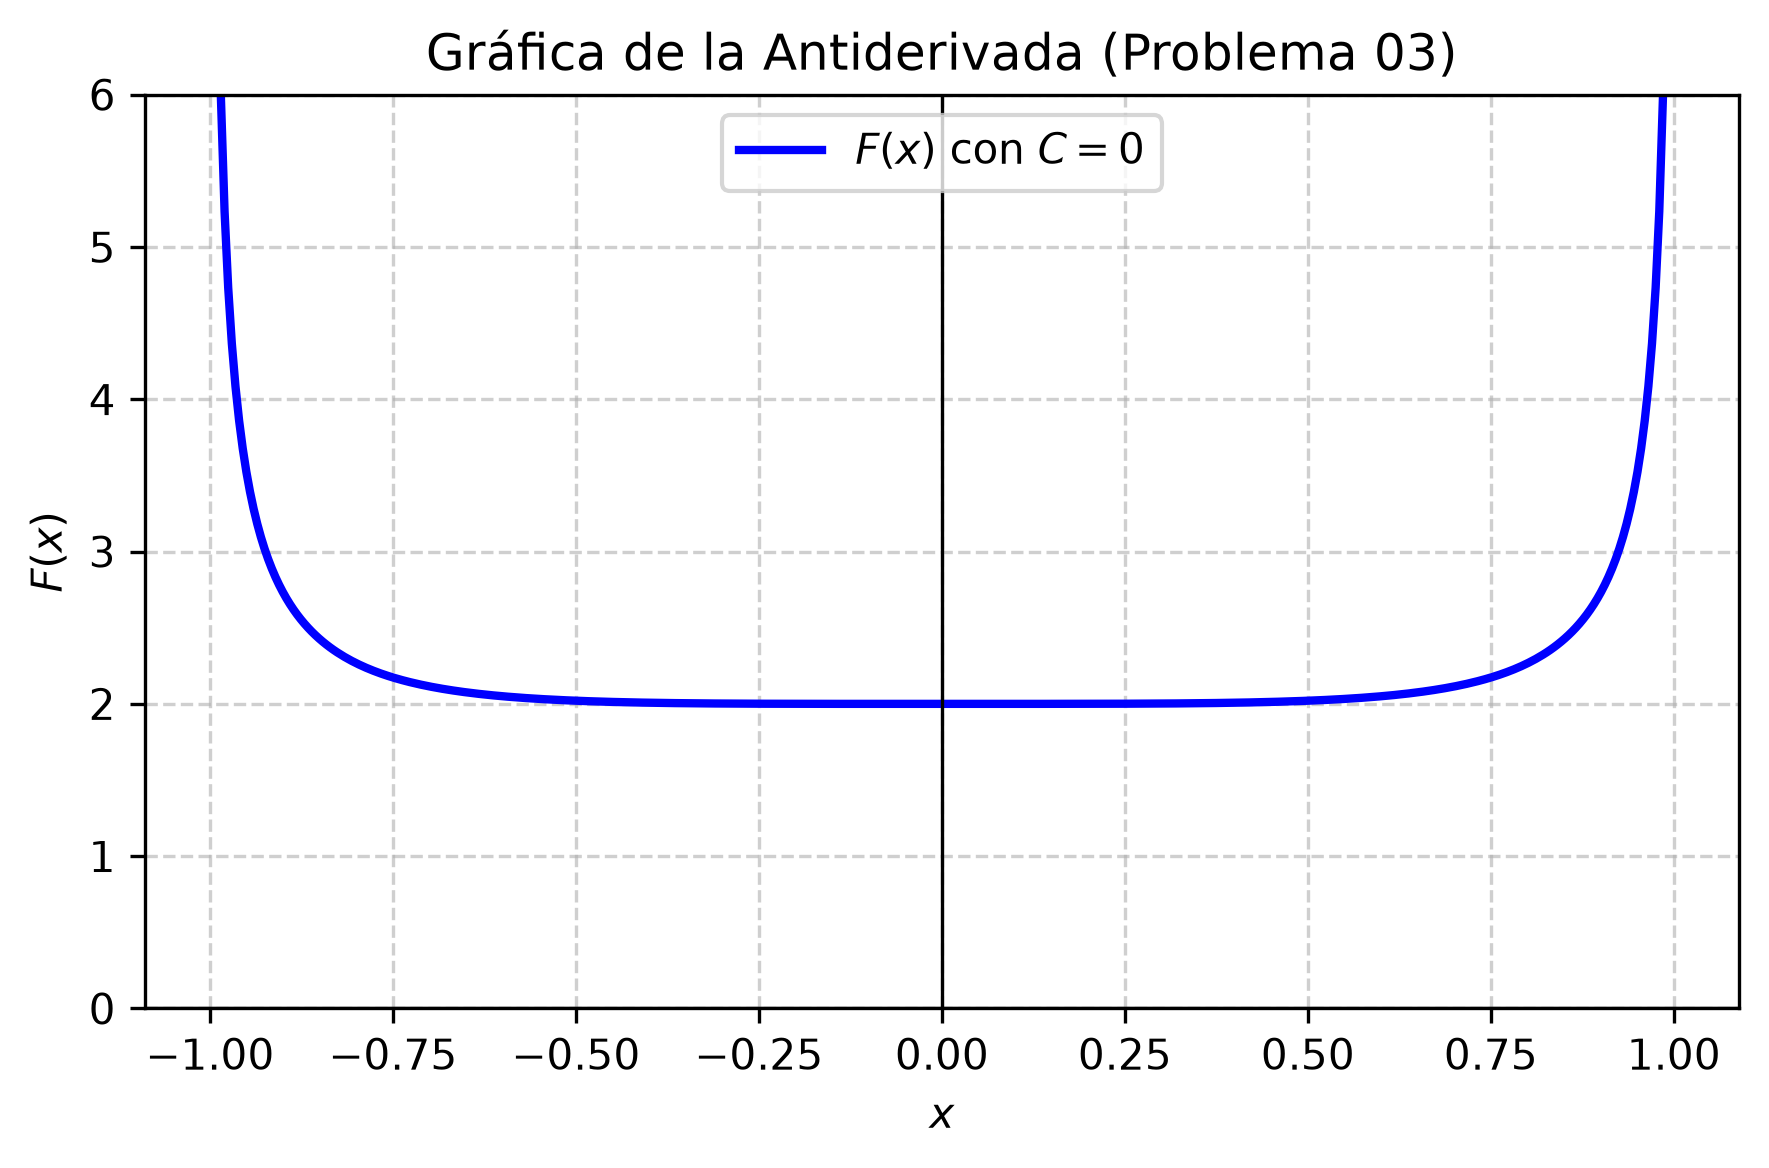
\includegraphics[width=\columnwidth]{semana_05/graficas/SEM05_P03_grafica.png}
	\caption{Representación gráfica de $f(x)$ y su antiderivada $F(x)$ evaluada para la constante de integración $C = 0$ (Problema 03).}
	\label{fig:problema03}
\end{figure}
